\documentclass[a4paper,14pt]{article}
\usepackage{blindtext}
\usepackage[T2A]{fontenc}
\usepackage[utf8]{inputenc}
\usepackage[english,russian]{babel}
\usepackage{listings}
\usepackage{geometry}
\usepackage{amssymb}
\usepackage{amsmath}
\usepackage[14pt]{extsizes}
\geometry{left=3cm}
\geometry{right=1.5cm}
\geometry{top=2cm}
\geometry{bottom=2cm}
\pagestyle{plain}
\usepackage{pgfplots}
\usepackage{filecontents}
\usepackage{graphicx}
\usepackage{indentfirst}
\DeclareGraphicsExtensions{.png}
\graphicspath{{images/}}
\usetikzlibrary{datavisualization}
\usetikzlibrary{datavisualization.formats.functions}
\usepackage{tabularx}
\pgfplotsset{width=7 cm}
\usepackage{xcolor}
%\renewcommand{\rmdefault}{ftm}
%\usepackage{mathptmx}
\usepackage{setspace}
% \usepackage{minted}

%\полуторный интервал
\onehalfspacing
\frenchspacing

\usepackage{tocloft}
\frenchspacing
\setcounter{page}{2}
\usepackage{multirow}
\usepackage{float}
\usepackage{multirow}

\renewcommand{\cftsecdotsep}{\cftdot}
\renewcommand{\cftsecleader}{\cftdotfill{\cftsecdotsep}}
\renewcommand{\cftsubsecleader}{\cftdotfill{\cftsecdotsep}}
\renewcommand{\cftsubsubsecleader}{\cftdotfill{\cftsecdotsep}}

%\renewcommand\cftchapdotsep{\cftdot}
%\renewcommand\cftsecdotsep{\cftdot}
%\renewcommand{\cftchapleader}{\cftdotfill{\cftchapdotsep}}

% Для измененных титулов глав:
% % подключаем нужные пакеты
%\definecolor{gray75}{gray}{0.75} % определяем цвет
%\newcommand{\hsp}{\hspace{20pt}} % длина линии в 20pt
% titleformat определяет стиль
%\titleformat{\chapter}[hang]{\Huge\bfseries}{\thechapter\hsp\textcolor{black}{|}\hsp}{0pt}{\Huge\bfseries}
%\usepackage{titlesec, blindtext, color}
%\titleformat{\chapter}[hang]{\Huge\bfseries}{\thechapter\hsp\textcolor{black}{|}\hsp}{0pt}{\Huge\bfseries}

\lstset{ %
extendedchars=\true,
inputencoding=utf8,
morekeywords={include, printf},
texcl=\true,
breaklines=\true,
escapeend=\end{russian},
escapechar=\%,
keepspaces=\true,
language=python,                 % выбор языка для подсветки
basicstyle=\small\sffamily, % размер и начертание шрифта для подсветки кода
numbers=left,               % где поставить нумерацию строк (слева\справа)
numberstyle=\tiny,           % размер шрифта для номеров строк
stepnumber=1,                   % размер шага между двумя номерами строк
numbersep=5pt,                % как далеко отстоят номера строк от подсвечиваемого кода
showspaces=\true,            % показывать или нет пробелы специальными отступами
showstringspaces=\true,      % показывать или нет пробелы в строках
showtabs=false,             % показывать или нет табуляцию в строках
frame=single,              % рисовать рамку вокруг кода
tabsize=4,                 % размер табуляции по умолчанию равен 2 пробелам
captionpos=t,              % позиция заголовка вверху [t] или внизу [b]
breaklines=true,           % автоматически переносить строки (да\нет)
breakatwhitespace=false, % переносить строки только если есть пробел
escapeinside={\#*}{*)}   % если нужно добавить комментарии в коде
}



\begin{document}
\pgfplotsset{compat=1.17}

\begin{titlepage}

    \begin{table}
        \centering
        \footnotesize
        \begin{tabular}{cc}
            \multirow{8}{*}{
\includegraphics[scale=0.35]{bmstu.jpg}}
            & \\
            & \\
            & \textbf{Министерство науки и высшего образования Российской Федерации} \\
            & \textbf{Федеральное государственное бюджетное образовательное учреждение} \\
            & \textbf{высшего образования} \\
            & \textbf{<<Московский государственный технический} \\
            & \textbf{университет имени Н.Э. Баумана>>} \\
            & \textbf{(МГТУ им. Н.Э. Баумана)} \\
        \end{tabular}
    \end{table}

    \vspace{-2.5cm}

    \begin{flushleft}
        \rule[-1cm]{\textwidth}{3pt}
        \rule{\textwidth}{1pt}
    \end{flushleft}

    \begin{flushleft}
		ФАКУЛЬТЕТ Информатика и системы управления 
	\end{flushleft}
        КАФЕДРА Программное обеспечение ЭВМ и информационные технологии

    \vspace{3cm}

    \begin{center}
		\textbf{Лабораторная работа № 3} \\
		\textbf{Дисциплина: <<Моделирование>>}
        \vspace{0.5cm}
	\end{center}

	\begin{center}
		\textbf{Тема: <<Программно-алгоритмическая реализация моделей на основе ОДУ второго порядка с краевыми условиями II и  III рода>>}
        \vspace{0.5cm}
    \end{center}

    \vspace{2cm}

	\begin{flushleft}
        \begin{tabular}{ll}
            \textbf{Студент} & Овчинникова А. П. \\
            \textbf{Группа} & ИУ7-65Б \\
            \textbf{Оценка (баллы)} & \\
            \textbf{Преподаватель} & Градов В.М.   \\
        \end{tabular}
    \end{flushleft}

    \vspace{2cm}

   \begin{center}
        Москва, 2020 г.
    \end{center}

\end{titlepage}

\setcounter{page}{2}

\subsection*{Цель работы}

Целью данной работы является получение навыков разработки  алгоритмов решения краевой задачи при реализации моделей, 
построенных на  ОДУ второго порядка.

\subsection*{Исходные данные}

1. Задана математическая модель.

Уравнение для функции $T(x)$:

\begin{equation}
	\frac{d}{dx} \left( k(x) \frac{dT}{dx} \right) - \frac{2}{R} \alpha(x) T + \frac{2T_0}{R} \alpha(x) = 0
\end{equation}

Краевые условия

\begin{equation}
	\begin{cases}
		x = 0, -k(0) \frac{dT}{dx} = F_0 \\
		x = l, -k(l) \frac{dT}{dx} = \alpha_N \left( T(l) - T_0 \right)
  	\end{cases}
\end{equation}

2. Функции $k(x), \alpha(x)$ заданы своими константами:
\begin{equation}
	k(x) = \frac{a}{x - b}
\end{equation}

\begin{equation}\
	\alpha(x) = \frac{c}{x - d}
\end{equation}

Константы $a, b$ следует найти из условий $k(0) = k_0, k(l) = k_N$, а константы
$c, d$ из условий $\alpha(0) = a_0, \alpha(l) = \alpha_N$. Величины
$k_0, k_N, \alpha_0, \alpha_N$ задает пользователь, их надо вынести в интерфейс.

3. Разностная схема с разностным краевым условием при $x = 0$.

\begin{equation}
	A_n y_{n+1} - B_n y_n + C_n y_{n-1} = - D_n, 1 \leq n \leq N -1
\end{equation}
где

$A_n = \frac{\chi_{n + \frac{1}{2}}}{h}$

$C_n = \frac{\chi_{n - \frac{1}{2}}}{h}$

$B_n = A_n + C_n + p_n h$

$D_n = f_n h$

Система (5) совместно с краевыми условиями решается методом прогонки.

Для величин $\chi_{N \pm 1/2}$ можно получить различные приближенные выражения,
численно вычисляя интеграл методом трапеций или методом средних.
Будем использовать метод средних:

\begin{equation}
	\chi_{N \pm 1/2} = \frac{k_n +  k_{n \pm 1}}{2}.
\end{equation}

Разностный аналог краевого условия при $x = 0$:

\begin{equation}
	y_0 = \frac{\chi_{\frac{1}{2}} - \frac{h^2}{8}p_{\frac{1}{2}}}{\chi_{\frac{1}{2}} + \frac{h^2}{8}p_{\frac{1}{2}} + \frac{h^2}{4}p_0} + \frac{h F_0 + \frac{h^2}{4} \left( f_{\frac{1}{2}} + f_0 \right)}{\chi_{\frac{1}{2}} + \frac{h^2}{8}p_{\frac{1}{2}} + \frac{h^2}{4}p_0}
\end{equation}

Примем простую аппроксимацию:

$p_{\frac{1}{2}} = \frac{p_0 + p_1}{2}$

$f_{\frac{1}{2}} = \frac{f_0 + f_1}{2}$

При получении разностного аналога краевого условия при 
$x = l$ интегро-интерполяционным методом необходимо учесть, что

\begin{equation}
	F_N = \alpha_N \left( y_N - T_0 \right)
\end{equation}

\begin{equation}
	F_{N-\frac{1}{2}} = \chi_{N-\frac{1}{2}}\frac{y_{N-1} - y_N}{h}.
\end{equation}



4. Значения параметров для отладки (все размерности согласованы) приведены в таблице 1.

\begin{table}[!h]
\caption{\label{tab.canonsummary} Значения параматров.}
\begin{center}
\begin{tabular}{|c c|}
\hline
$k_0 = $ & 0.4 Вт/см К \\
$k_N = $ & 0.1 Вт/см К \\
$\alpha_0 = $ & 0.05 Вт/см$^2$ К \\
$\alpha_N = $ & 0.01 Вт/см$^2$ К \\
$l = $ & 10 см \\
$T_0 = $ & 300 К \\
$R = $ & 0.5 см \\
$F_0 = $ & 50 Вт/см$^2$ \\
\hline
\end{tabular}
\end{center}
\end{table} 

\subsection*{Физическое содержание задачи}

Сформулированная математическая модель описывает температурное поле
$T(x)$ вдоль  цилиндрического стержня радиуса $R$ и длины $l$,
причем $R << l$ и температуру можно принять постоянной по радиусу цилиндра.
Ось $X$ направлена вдоль оси цилиндра и начало координат совпадает с левым торцем стержня.
Слева при $x = 0$ цилиндр нагружается тепловым потоком $F_0$.
тержень обдувается воздухом, температура которого равна $T_0$.
В результате происходит съем тепла с цилиндрической поверхности и поверхности правого торца при $x = l$.
Функции $k(x), \alpha(x)$ являются, соответственно, коэффициентами теплопроводности материала стержня и теплоотдачи при обдуве. 

\subsection*{Задание}

\begin{enumerate}
	\item Представить разностный аналог краевого условия при $x = l$ и его краткий вывод интегро-интерполяционным методом.
	\item График зависимости температуры $T(x)$ от координаты $X$ при заданных выше параметрах.
	\item График зависимости $T(x)$ при $F_0 = -10$ Вт/см$^2$.
	Справка. При отрицательном тепловом потоке слева идет съем тепла, поэтому производная
	$T'(x)$ должна быть положительной.
	\item График зависимости $T(x)$ при увеличенных значениях $\alpha(x)$ (например, в 3 раза). Сравнить с п.2.
		  Справка. При увеличении теплосъема и неизменном потоке $F_0$ уровень температур $T(x)$ должен снижаться, а градиент  увеличиваться.
	\item График зависимости $T(x)$ при $F_0 = 0$.
	Справка. В данных условиях тепловое нагружение отсутствует, причин для нагрева нет, температура стержня должна быть равна температуре окружающей среды
	$T_0$ (разумеется с некоторой погрешностью, определяемой приближенным характером вычислений).
\end{enumerate}


\subsection*{Предварительные вычисления}

1. Константы $a, b, c, d$:

$k_0 = -\frac{a}{b} \Rightarrow a = - k_o b$

$k_N = - \frac{a}{l - b} \Rightarrow b = \frac{k_N l}{k_N - k_0}$

$\alpha_0 = - \frac{c}{d} \Rightarrow c = - \alpha_0d$

$\alpha_N = \frac{c}{l - d} \Rightarrow d = \frac{\alpha_N l}{\alpha_N - \alpha_0}$.

2. Разностный аналог краевого условия при $x = l$:

Пусть $p(x) = \frac{2}{R}\alpha(x)$, $f(x) = \frac{2T_0}{R}\alpha(x)$.
Тогда имеем квазилинейное уравнение:

\begin{equation}
	\frac{d}{dx} \left( k(x) \frac{dT}{dx} \right) - p(x) T + f(x) = 0
\end{equation}

Краевое условие справа III рода:

$x = l, -k(l)\frac{dT}{dx} = \alpha_N(T(l) - T_0)$

Получим разностный аналог краевого условия при $x = l$.

Примем $F = -k(x)\frac{dT}{dx}$

Проинтегрируем уравнение 9 на отрезке $[x_{N-1/2}; x_N]$:

\begin{equation}
	-\int\limits_{x_{N-1/2}}^{x_N} \frac{dF}{dx} dx -
	\int\limits_{x_{N-1/2}}^{x_N} p(x)T dx + 
	\int\limits_{x_{N-1/2}}^{x_N} f(x) dx = 0
\end{equation}

Второй и третий интегралы вычислим методом трапеций:

\begin{equation}
	-(F_N - F_{N - 1/2}) -\frac{h}{4}(p_N y_N + p_{N-1/2}y_{N-1/2})
	+ \frac{h}{4}(f_N + f_{N-1/2}) = 0
\end{equation}

Примем простую аппроксимацию $y_{N-1/2} = \frac{y_{N-1} + y_N}{2}$ 
и применим (7), (8) к (11):

\begin{eqnarray}
	-\left[ \alpha_N(y_N - T_0) - \chi_{N-1/2}\frac{y_{N-1} - y_N}{h} \right] - \nonumber \\
	- \frac{h}{4} \left( p_N y_N + p_{N-1/2}\frac{y_N + t_{N-1}}{2} \right) + \nonumber \\
	+ \frac{h}{4} \left( f_N + f_{N-1/2} \right) = 0
\end{eqnarray}

Из (12) получаем:

\begin{eqnarray}
	y_{N-1} \left( \frac{\chi_{N-1/2}}{h}  - \frac{hp_{N-1/2}}{8} \right) + \nonumber \\
	+ y_N \left( -\alpha_N - \frac{\chi_{N-1/2}}{h} - \frac{hp_N}{4} - \frac{hp_{N-1/2}}{8} \right) = \nonumber \\
	= -\alpha_N T_0 - \frac{h}{4} \left( f_N + f_{N-1/2} \right)
\end{eqnarray}

Можно принять простую аппроксимацию:

$p_{N-1/2} = \frac{p_N + p_{N-1}}{2}$

$f_{N-1/2} = \frac{f_N + f_{N-1}}{2}$.

Тогда:

\begin{eqnarray}
	y_{N-1} \left( \frac{\chi_{N-1/2}}{h} - \frac{h}{8} \cdot \frac{p_N + p_{N-1}}{2} \right) + \nonumber \\
	y_N \left( -\alpha_N - \frac{\chi_{N-1/2}}{h} - \frac{hp_N}{4} - \frac{h}{8} \cdot \frac{p_N + p_{N-1}}{2} \right) = \nonumber \\
	= - \alpha_N T_0 - \frac{h}{4} \left( f_N + \frac{f_N + f_{N-1}}{2} \right)
\end{eqnarray}

\subsection*{Код программы}

Код программы представлен в листингах 1-2.

\begin{lstlisting}[label=code1,caption=\text{Класс MyApp.}]
	import sys

	from PyQt5 import QtWidgets
	from PyQt5.QtWidgets import QMessageBox
	
	from Ui_MainWindow import Ui_MainWindow
	
	from Modeller import Modeller
	
	class MyApp(QtWidgets.QMainWindow):
		def __init__(self):
			super(MyApp, self).__init__()
			self.ui = Ui_MainWindow()
			self.ui.setupUi(self)
	
			self.ui.set_def_button.clicked.connect(self.set_defaults)
			self.ui.run_button.clicked.connect(self.run)
	
			self.defaults = {
				"k0" : 0.4,
				"kN" : 0.1,
				"a0" : 0.05,
				"aN" : 0.01,
				"l"  : 10,
				"T0" : 300,
				"R"  : 0.5,
				"F0" : 50,
				"h"  : 0.1
			}
	
			self.data = {
				"k0" : None,
				"kN" : None,
				"a0" : None,
				"aN" : None,
				"l"  : None,
				"T0" : None,
				"R"  : None,
				"F0" : None,
				"h"  : None
			}
	
			self.set_defaults()
		
		def set_defaults(self):
			self.ui.lineEdit_k0.setText(str(self.defaults.get("k0")))
			self.ui.lineEdit_kN.setText(str(self.defaults.get("kN")))
			self.ui.lineEdit_alpha0.setText(str(self.defaults.get("a0")))
			self.ui.lineEdit_alphaN.setText(str(self.defaults.get("aN")))
			self.ui.lineEdit_l.setText(str(self.defaults.get("l")))
			self.ui.lineEdit_T0.setText(str(self.defaults.get("T0")))
			self.ui.lineEdit_R.setText(str(self.defaults.get("R")))
			self.ui.lineEdit_F0.setText(str(self.defaults.get("F0")))
			self.ui.lineEdit_h.setText(str(self.defaults.get("h")))
	
		def get_data(self):
			try:
				self.data["k0"] = float(self.ui.lineEdit_k0.text())
				self.data["kN"] = float(self.ui.lineEdit_kN.text())
				self.data["a0"] = float(self.ui.lineEdit_alpha0.text())
				self.data["aN"] = float(self.ui.lineEdit_alphaN.text())
				self.data["l"] = float(self.ui.lineEdit_l.text())
				self.data["T0"] = float(self.ui.lineEdit_T0.text())
				self.data["R"] = float(self.ui.lineEdit_R.text())
				self.data["F0"] = float(self.ui.lineEdit_F0.text())
				self.data["h"] = float(self.ui.lineEdit_h.text())
			except ValueError:
				return False
			return True
	
		def run(self):
			if self.get_data():
				print("Computing...")
				mdlr = Modeller(self.data)
				mdlr.compute()
				print("Finish.")
			else:
				self.msg_box("Error!", "Error! Incorrect input!", QMessageBox.Critical)
	
		def msg_box(self, title, message, type):
			msg = QMessageBox(self)
			msg.setIcon(type)
			msg.setWindowTitle(title)
			msg.setText(message)
			msg.addButton('Ok', QMessageBox.AcceptRole)
			msg.exec()
	
	
	def main():
		app = QtWidgets.QApplication(sys.argv)
		window = MyApp()
		window.show()
		app.exec_()
	
	
	if __name__ == '__main__':
		main()	
\end{lstlisting}

\begin{lstlisting}[label=code1,caption=\text{Класс Modeller.}]
	import matplotlib.pyplot as plt

	class Modeller():
		def __init__(self, data):
			self.data = data
	
			self.k0 = self.data.get("k0")
			self.kN = self.data.get("kN")
			self.a0 = self.data.get("a0")
			self.aN = self.data.get("aN")
			self.l = self.data.get("l")
			self.T0 = self.data.get("T0")
			self.R = self.data.get("R")
			self.F0 = self.data.get("F0")
			self.h = self.data.get("h")
	
			self.start_l = 0
	
			self.b = (self.kN * self.l) / (self.kN - self.k0)
			self.a = - self.k0 * self.b
			self.d = (self.aN * self.l) / (self.aN - self.a0)
			self.c = - self.a0 * self.d
	
			self.M0, self.K0, self.P0 = self.left_boundary_condition()
			self.MN, self.KN, self.PN = self.right_boundary_condition()
	
		# приближенно	вычислим	интеграл	методом	средних
		def chi_plus_half(self, func, x):
			return (func(x) + func(x + self.h)) / 2
		
		# приближенно	вычислим	интеграл	методом	средних
		def chi_minus_half(self, func, x):
			return (func(x) + func(x - self.h)) / 2
	
		def right_boundary_condition(self):
			chi = self.chi_minus_half(self.k, self.l)
	
			pn = self.p(self.l)
			fn = self.f(self.l)
	
			pn12 = (pn + self.p(self.start_l - self.h)) / 2
			fn12 = (fn + self.f(self.start_l - self.h)) / 2
	
			MN = chi / self.h - (self.h * pn12) / 8
			KN = -self.aN - chi / self.h - (self.h * pn) / 4 - (self.h * pn12) / 8
			PN = - self.aN * self.T0 - self.h / 4 * (fn + fn12)
	
			return MN, KN, PN
			
		def left_boundary_condition(self):
			chi = self.chi_minus_half(self.k, self.start_l)
			h_2 = self.h ** 2
			p0 = self.p(self.start_l)
			f0 = self.f(self.start_l)
			p12 = (p0 + self.p(self.start_l + self.h)) / 2
			f12 = (f0 + self.f(self.start_l + self.h)) / 2
			M0 = - chi + h_2 / 8 * p12
			K0 = chi + h_2 / 8 * p12 + h_2 / 4 * p0
			P0 = self.h * self.F0 + h_2 / 4 * (f12 + f0)
	
			return M0, K0, P0
	
		def compute(self):
			epsilon = [0, - self.M0 / self.K0]
			eta = [0, self.P0 / self.K0]
			xes = [0, self.h]
	
			# вычисляем	значения	прогоночных	коэффицентов
			x = self.h
			n = 1
			while x + self.h < self.l:
				newEps = self.C(x) / (self.B(x) - self.A(x) * epsilon[n])
				epsilon.append(newEps)
	
				newEta = (self.D(x) + self.A(x) * eta[n]) / (self.B(x) - self.A(x) * epsilon[n])
				eta.append(newEta)
	
				x += self.h
				n += 1
				xes.append(x)
	
			# обратный	ход
	
			T = [0] * (n + 1)
			T[n] = (self.PN - self.MN * eta[n]) / (self.KN + self.MN * epsilon[n])
	
			for i in range(n-1, -1, -1):
				T[i] = epsilon[i + 1] *T[i + 1] + eta[i+1]
	
			self.plot1(xes, T)
	
		def plot1(self, x, y):
			print(y)
			plt.plot(x, y)
			plt.xlabel("x, cm")
			plt.ylabel("t, K")
			plt.grid()
			plt.show()
		
		def p(self, x):
			return (2 * self.alpha(x)) / self.R
	
		def f(self, x):
			return (2 * self.T0 * self.alpha(x)) / self.R
	
		def k(self, x):
			return self.a / (x - self.b)
	
		def alpha(self, x):
			return self.c / (x - self.d)
	
		def A(self, n):
			return self.chi_plus_half(self.k, n) / self.h
	
		def C(self, n):
			return self.chi_minus_half(self.k, n) / self.h
	
		def B(self, n):
			return self.A(n) + self.C(n) + self.p(n) * self.h
	
		def D(self, n):
			return self.f(n) * self.h	
\end{lstlisting}

\newpage
\subsection*{Результаты работы программы}

1. Краткий вывод разностного аналога краевого условия
при $x = l$ представлен в разделе "Предварительные вычисления".

2. График зависимости температуры $T(x)$ от координаты $X$ при заданных выше параметрах (рисунок 1).

\begin{figure}[!h]
\center{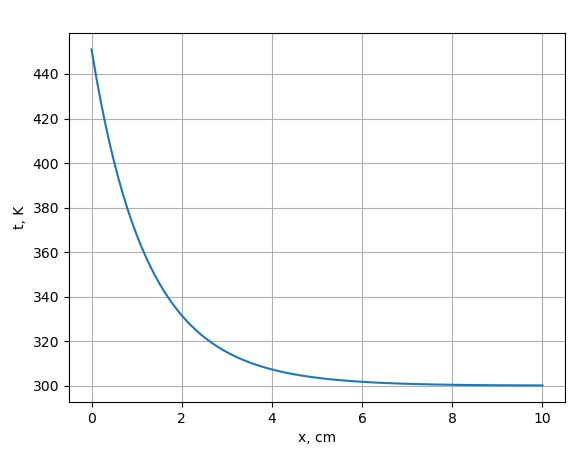
\includegraphics[width=14cm]{gr1}}
\caption{График зависимости температуры $T(x)$ от координаты $X$ при параметрах по умолчанию.}
\label{fig:image}
\end{figure}

\newpage
3. График зависимости $T(x)$ при $F_0 = -10$ Вт/см$^2$.
Справка. При отрицательном тепловом потоке слева идет съем тепла, поэтому производная
$T'(x)$ должна быть положительной (рисунок 2).

\begin{figure}[!h]
	\center{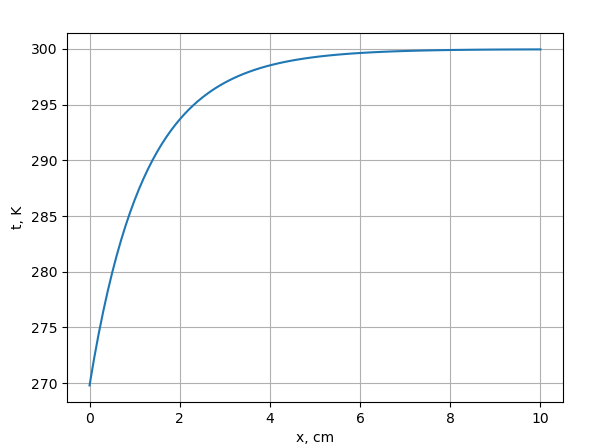
\includegraphics[width=14cm]{gr2}}
	\caption{График зависимости $T(x)$ при $F_0 = -10$ Вт/см$^2$.}
	\label{fig:image}
\end{figure}

\newpage
4. График зависимости $T(x)$ при увеличенных значениях $\alpha(x)$ (например, в 3 раза). Сравнить с п.2.
Справка. При увеличении теплосъема и неизменном потоке $F_0$ уровень температур $T(x)$ должен снижаться, а градиент  увеличиваться (рисунки 3-4).

\begin{figure}[!h]
	\center{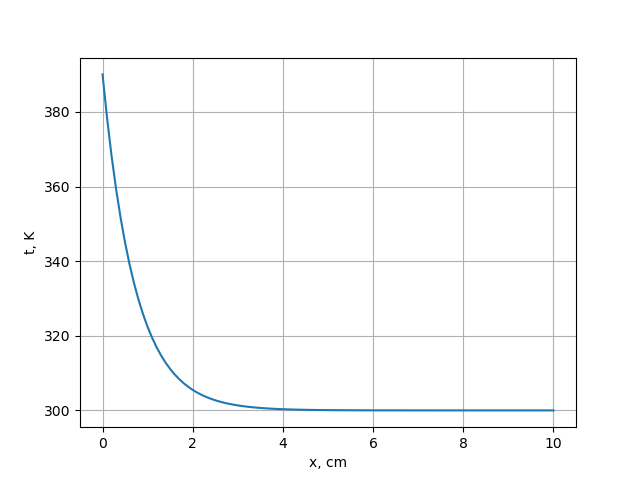
\includegraphics[width=12cm]{Figure_1}}
	\caption{График зависимости $T(x)$ при увеличенных значениях $\alpha(x)$ (в 3 раза).}
	\label{fig:image}
\end{figure}

\begin{figure}[!h]
	\center{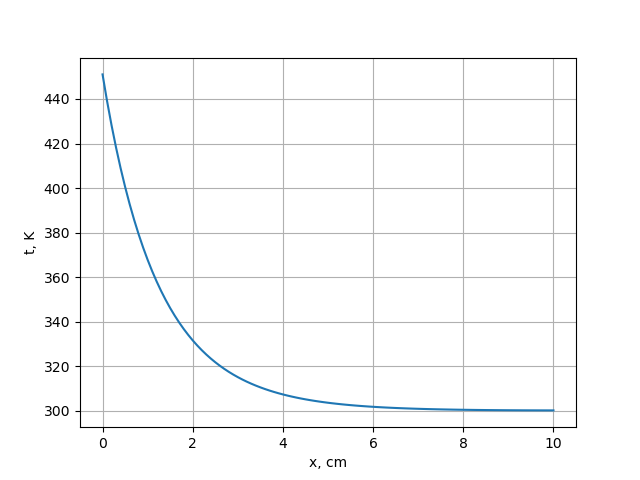
\includegraphics[width=12cm]{Figure_2}}
	\caption{График зависимости $T(x)$ при стандартных параметрах.}
	\label{fig:image}
\end{figure}

Если увеличить значение $\alpha(x)$ в 100 раз, то уровень температур будет снижаться быстрее (рисунок 5).

\begin{figure}[!h]
	\center{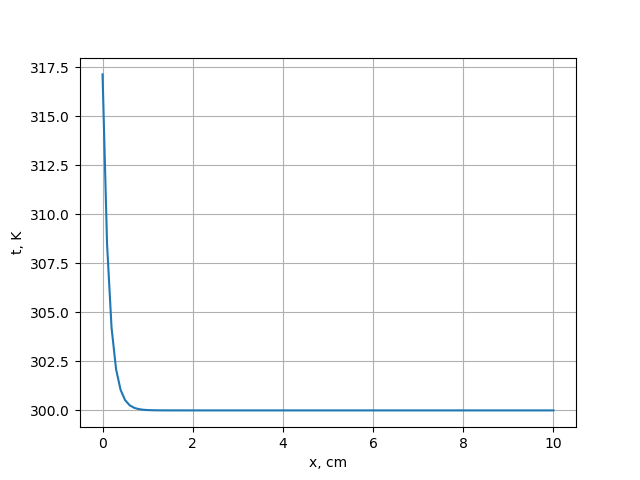
\includegraphics[width=12cm]{scale100}}
	\caption{График зависимости $T(x)$ при увеличенных значениях $\alpha(x)$ (в 100 раз).}
	\label{fig:image}
\end{figure}

\newpage
5. График зависимости $T(x)$ при $F_0 = 0$.
Справка. В данных условиях тепловое нагружение отсутствует, причин для нагрева нет, температура стержня должна быть равна температуре окружающей среды
$T_0$ (разумеется с некоторой погрешностью, определяемой приближенным характером вычислений) (рисунки 6-7).

\begin{figure}[!h]
	\center{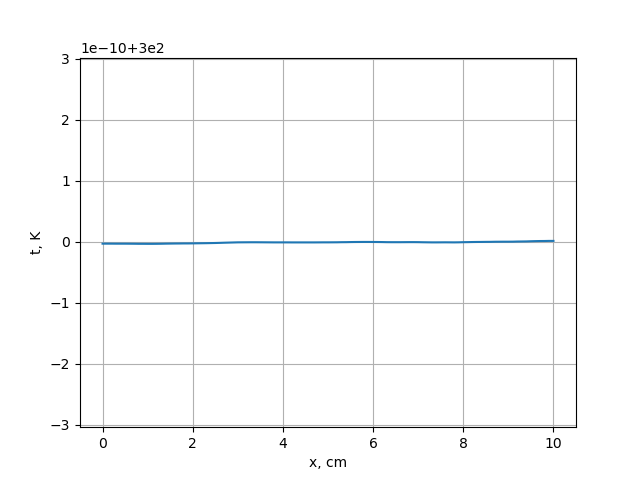
\includegraphics[width=15cm]{f00}}
	\caption{График зависимости $T(x)$ при $F_0 = 0$ (шаг 0.01).}
	\label{fig:image}
\end{figure}

Если уменьшить шаг, то можно увидеть погрешность (рисунок 7).

\begin{figure}[!h]
	\center{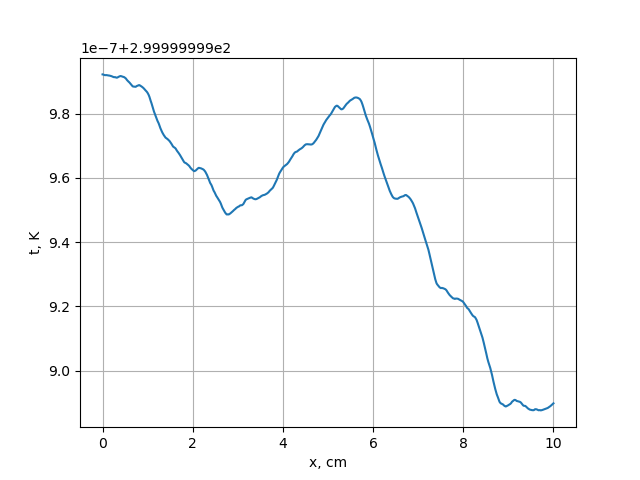
\includegraphics[width=15cm]{err}}
	\caption{График зависимости $T(x)$ при $F_0 = 0$ (шаш 0.0001).}
	\label{fig:image}
\end{figure}

\newpage
\subsection*{Ответы на вопросы}

\textbf{1. Какие способы тестирования программы можно предложить?}

Правильность работы программы можно определить по виду графиков.
Графики должны соответствовать физическому смыслу задачи.

Например, в п. 5 задания к лабораторной работе (рисунки 6-7) программа
тестировалась при $F_0 = 0$. Температура стержня равна температуре
окружающей среды ($F_0 = T_0$), т.к. в данных условиях тепловое нагружение
отсутствует и причин для нагревва нет. График на рисунках 6-7 соответствует 
физическому смыслу задачи.

Другие графики из задания к лабораторной работе также соответсвуют
физическому смыслу задачи (см. справку к графикам).

\textbf{2. Получите  простейший разностный аналог нелинейного краевого условия при $x = l$:
$x = l, -k(l)\frac{dT}{dx} = \alpha_N(T(l) - T_0) + \varphi (T)$, где 
$\varphi(T)$ -- заданная функция. Производную аппроксимируйте односторонней разностью.}

Примем простейшую аппроксимацию

\begin{eqnarray}
	\frac{dT}{dx} = \frac{T(x + \Delta x) - T(x)}{\Delta x}
\end{eqnarray}

Подставляя (16) в исходное уравнение при $x = l$ получим:

\begin{eqnarray}
	-k_l \frac{T_l -T_{l-1}}{\Delta x} = \alpha_N(T_l - T_0) + \varphi(T_l)
\end{eqnarray}

\textbf{3. Опишите алгоритм применения метода прогонки, если при $x = 0$ 
краевое условие линейное (как в настоящей работе), а при $x = l$, как в п.2.}

Имеем систему уравнений:

\begin{equation*}
	\begin{cases}
		A_n y_{n+1} - B_n y_n + C_n y_{n-1} = - D_n, 1 \leq n \leq N -1 \\
		%y_0 = \frac{\chi_{\frac{1}{2}} - \frac{h^2}{8}p_{\frac{1}{2}}}{\chi_{\frac{1}{2}} + \frac{h^2}{8}p_{\frac{1}{2}} + \frac{h^2}{4}p_0} + \frac{h F_0 + \frac{h^2}{4} \left( f_{\frac{1}{2}} + f_0 \right)}{\chi_{\frac{1}{2}} + \frac{h^2}{8}p_{\frac{1}{2}} + \frac{h^2}{4}p_0}
		x = 0, -k(0) \frac{dT}{dx} = F_0 \\
		x = l, -k(l) \frac{dT}{dx} = \alpha_N \left( T(l) - T_0 \right)
	\end{cases}
\end{equation*}

Т. к. можно определить начальные значения прогоночиных коэффициентов,
будем использовать правую прогонку.

Принимая простейшую (первого порядка точности) аппроксимацию краевого
условия при $x = 0$, получим его разностный аналог

\begin{equation}
	T_0 = T_1 + \frac{F_0 h}{k_0}.
\end{equation}

Из (19) найдем начальные прогоночные коэффициенты:

\begin{eqnarray}
	\varepsilon_1 = 1 \nonumber \\
	\eta_1 = \frac{F_0 h}{k_0}.
\end{eqnarray}

Рекуррентные соотношения для определения прогоночных коэффициентов:

\begin{eqnarray}
	\varepsilon_{n+1} = \frac{C_n}{B_n - A_n \varepsilon_n} \\
	\eta_{n+1} = \frac{D_n + A_n \eta_n}{B_n - A_n \varepsilon_n}
\end{eqnarray}

Имея (20), по (21) и (22) находим прогоночные коэффициенты.
После этого делаем обратный ход. 

Чтобы в обратном ходе найти все значения $T_n$, надо знать $T_N$.
Найдем $T_N$.

Основная прогоночная формула имеет вид:

\begin{equation}
	T_{n-1} = \varepsilon_n T_n + \eta_{n}.
\end{equation}

Из (23) и (18) находим:

\begin{eqnarray}
	-k_N \frac{T_N - T_{N-1}}{h} = \alpha_N(T_N - T_0) + \varphi(T_n)
\end{eqnarray}

\begin{eqnarray}
	-k_N \frac{T_n - (\varepsilon_N T_N + \eta_N)}{h} = \alpha_N(T_N - T_0) + \varphi(T_n)
\end{eqnarray}

\begin{eqnarray}
	T_N \left( -k_N + k_N \varepsilon_N - h \alpha_N \right) = -k_N \eta_N - h \alpha_N T_0 + \varphi(T_N) h
\end{eqnarray}

Решение уравнения (26) можно найти методом дихотомии.

Таким образом, метод прогонки содержит два этапа:

\begin{itemize}
	\item Прямой ход. По формулам (20) определяем начальные значения
		  прогоночных коэффициентов. По формулам (21) и (22) вычисляем массивы прогоночных
		  коэффициентов.
	\item Обратный ход. По формуле (26) определяем $T_N$ значение неизвестной функции в последней точке.
		  Далее по формуле (23) находим все значения $T_n$.
\end{itemize}

\textbf{4. Опишите алгоритм определения единственного значения сеточной функции
$y_p$ в одной заданной точке $p$. Использовать встречную прогонку,
т.е. комбинацию правой и левой прогонок (лекция №8). 
Краевые условия линейные.}

В правой прогонке начальные прогоночные коэффициенты находятся
по формуле (19), рекурентные соотношения для определения остальных прогоночных
коэффициентов -- (21) и (22). Основная прогоночная формула -- (23).

В левой прогонке рекурентные соотношения для определения прогоночных коэффициентов (обозначим их $\alpha$ и $\beta)$:

\begin{equation}
	\alpha_{n-1} = \frac{C_n}{B_n - A_n \alpha_n}
\end{equation}

\begin{equation}
	\beta_{n-1} = \frac{A_n\beta_n + D_n}{B_n - A_n \alpha_n}.
\end{equation}

Основная прогоночная формула для левой прогонки:

\begin{equation}
	T_n = \alpha_{n-1} T_{n-1} + \beta_{n-1}.
\end{equation}

Объединив левую и правую прогонки, получим:

\begin{equation}
	\begin{cases}
		T_p = \alpha_{p-1} T_{p-1} + \beta_{p-1} \\
		T_{p-1} = \varepsilon_p T_p + \eta_{p}
	\end{cases}
\end{equation}

Подставив второе уравнение в первое, получим:

\begin{equation}
	T_p = \frac{\alpha_{p-1} \eta_p + \beta_{p-1}}{1 - \alpha_{p-1} \varepsilon_p}
\end{equation}

\subsection*{Вывод}

Таким образом, в ходе данной работы были получены навыки разработки 
алгоритмов решения краевой задачи при реализации моделей, 
построенных на  ОДУ второго порядка.

\end{document}

\end{document}